% This is samplepaper.tex, a sample chapter demonstrating the
% LLNCS macro package for Springer Computer Science proceedings;
% Version 2.20 of 2017/10/04
%
\documentclass[runningheads]{llncs}
%
\usepackage{booktabs}
\usepackage{graphicx}
\usepackage{pgfplots}
\usepackage{tikz}
\usepackage{enumitem}
\usepackage{gensymb}
\usepackage{amsmath}
\usepgfplotslibrary{clickable}
\usetikzlibrary{shapes,arrows,positioning,fit,backgrounds,matrix,chains,patterns,trees,calc,arrows.meta}

\usepackage{textcomp}
\usepackage{amssymb}
\usepackage{xspace}

\newcommand{\tickYes}{\checkmark}
\newcommand{\tickNo}{\textsl{\textsf{X}}}
\newcommand{\ntextnumero}{{\fontfamily{txr}\selectfont \textnumero}\xspace}

\newcommand{\Iris}{\ensuremath{\mathbf{I}}}
\newcommand{\Lits}{\ensuremath{\mathbf{L}}}
\newcommand{\Bnodes}{\ensuremath{\mathbf{B}}}
\newcommand{\Vars}{\ensuremath{\mathbf{V}}}

\newcommand{\da}{\ensuremath{:\nolinebreak\mkern-1.2mu\nolinebreak=}}

\newcommand{\ah}[1]{{\color{blue}\textsc{ah:} #1}}

\usepackage{xcolor}
\usepackage{hyperref}
\definecolor{dark-blue}{rgb}{0.0,0.0,0.2}
\definecolor{dark-green}{rgb}{0.0,0.2,0.0}
\definecolor{dark-red}{rgb}{0.2,0.0,0.0}
\hypersetup{
    colorlinks, linkcolor={dark-red},
    citecolor={dark-green}, urlcolor={dark-blue},
    pdftitle={Estimating the dynamics of SPARQL query results},    % title
%    pdfauthor={Alberto Moya, Aidan Hogan},     % author
    pdfsubject={ISWC 2019},   % subject of the document
    pdfkeywords={SPARQL;} {Linked Data;} {Dynamics;} {Wikidata;}, % list of keywords
}


%%%%%%%%%%%%%%%%%%%%%%%%%%%%%%%%%%%%%%%%%%%%%%%%%
% SPARQL Listing style
%%%%%%%%%%%%%%%%%%%%%%%%%%%%%%%%%%%%%%%%%%%%%%%%%
\usepackage{listings}

\colorlet{punct}{red!60!black}
\definecolor{background}{HTML}{EEEEEE}
\definecolor{delim}{RGB}{120,20,40}
\definecolor{keyw}{RGB}{0,0,192}
\definecolor{stri}{RGB}{100,0,130}
\colorlet{numb}{magenta!60!black}

\lstdefinelanguage{sparql}{
	sensitive=false,
	extendedchars=true,
	literate={á}{{\'a}}1 {é}{{\'e}}1 {í}{{\'{\i}}}1 {ó}{{\'o}}1 {ú}{{\'u}}1
	{Á}{{\'A}}1 {É}{{\'E}}1 {Í}{{\'I}}1 {Ó}{{\'O}}1 {Ú}{{\'U}}1
	{ü}{{\"u}}1 {Ü}{{\"U}}1 {ñ}{{\~n}}1 {Ñ}{{\~N}}1 {¿}{{?``}}1 {¡}{{!``}}1
	{<}{{{\color{delim}<}}}{1}
	{>}{{{\color{delim}>}}}{1}
	{?}{{{\color{delim}?}}}{1}
	{*}{{{\color{delim}*}}}{1}
	{+}{{{\color{delim}+}}}{1}
	{/}{{{\color{delim}/}}}{1}
	{,}{{{\color{punct}{,}}}}{1}
	{;}{{{\color{punct}{;}}}}{1}
	{.}{{{\color{punct}{.}}}}{1}
	{:}{{{\color{punct}{:}}}}{1}
	{\{}{{{\color{delim}{\{}}}}{1} {\}}{{{\color{delim}{\}}}}}{1}
	{(}{{{\color{punct}(}}}{1} {)}{{{\color{punct})}}}{1},
	morekeywords={ask,select,from,where,order,by,distinct,limit,offset,optional,union,filter,prefix,bound,desc,lang,regex,str,group,not,exists,minus,service,certain,maybe,coalesce,bind,as,strafter}
}

\lstdefinestyle{sparqld}{
	basicstyle=\scriptsize\ttfamily,
	identifierstyle=\color{black},
	keywordstyle=\color{keyw}\bfseries,
	ndkeywordstyle=\color{greenCode}\bfseries,
	stringstyle=\color{stri}\ttfamily,
	commentstyle=\color{gray}\ttfamily,
	language={sparql},
	tabsize=2,
	showtabs=false,
	showspaces=false,
	showstringspaces=false,
	extendedchars=true,
	escapechar=`,
	frame={single},
	breaklines=true,
	basewidth=0.5em,
	comment=[l]{\#},
	morestring=[b]",
	moredelim=[is][\color{magenta}]{~}{~},
	moredelim=**[is][\color{gray}]{£}{£},
	moredelim=**[is][\color{blue!50!black}]{$}{$},
	moredelim=**[is][\color{green!50!black}]{¬}{¬},
	xleftmargin=2ex,
	xrightmargin=1ex,
	aboveskip=1.5ex,
	belowskip=1.5ex
}

\makeatletter
\newcommand{\sqbox}{%
	\collectbox{%
		\@tempdima=\dimexpr\width-\totalheight\relax
		\ifdim\@tempdima<\z@
		\fbox{\hbox{\hspace{-.5\@tempdima}\BOXCONTENT\hspace{-.5\@tempdima}}}%
		\else
		\ht\collectedbox=\dimexpr\ht\collectedbox+.5\@tempdima\relax
		\dp\collectedbox=\dimexpr\dp\collectedbox+.5\@tempdima\relax
		\fbox{\BOXCONTENT}%
		\fi
	}%
}
\makeatother
%%%%%%%%%%%%%%%%%%%%%%%%%%%%%%%%%%%%%%%%%%%%%%%%%
% /SPARQL Listing style
%%%%%%%%%%%%%%%%%%%%%%%%%%%%%%%%%%%%%%%%%%%%%%%%%

%\usepackage{floatrow}
% Table float box with bottom caption, box width adjusted to content
%\newfloatcommand{capbtabbox}{table}[][\FBwidth]


\usepackage{listings}
\lstset{language=SQL,morekeywords={PREFIX,java,rdf,rdfs,url}}
% Used for displaying a sample figure. If possible, figure files should
% be included in EPS format.
%
% If you use the hyperref package, please uncomment the following line
% to display URLs in blue roman font according to Springer's eBook style:
% \renewcommand\UrlFont{\color{blue}\rmfamily}

\begin{document}
%
\title{Estimating the dynamics of SPARQL query results
%\thanks{This work was supported by CONICYT PFCHA, Doctorado Becas Chile/2017 -- 72180000, the Millennium Institute for Foundational Research on Data (IMFD) and FONDECYT Grant No. 1181896.}
}
%
%\titlerunning{Abbreviated paper title}
% If the paper title is too long for the running head, you can set
% an abbreviated paper title here
%
%\author{Alberto Moya\orcidID{0000-0002-7003-5087} \and 
%Aidan Hogan\orcidID{0000-0001-9482-1982}}
%
%\authorrunning{A. Moya and A. Hogan}
% First names are abbreviated in the running head.
% If there are more than two authors, 'et al.' is used.
%
%\institute{IMFD; DCC, University of Chile\\
%\email{\{amoya,ahogan\}@dcc.uhile.cl}}
%
\maketitle              % typeset the header of the contribution
%
\begin{abstract}
We address the problem of estimating when the results of an input SPARQL query results over dynamic RDF datasets will change. We propose a framework that extracts features from the query and/or from past versions of the target dataset. The resulting features are then used to predict (1) whether or not the results for a query will change in the near future using classifiers, and (2) when they might change (if at all) using linear regression. To evaluate our proposal, we create a gold standard based on 23 versions of Wikidata and a curated collection of 221 SPARQL queries. Our results show that the quality of predictions using query features and lightweight statistics of the dynamics of individual predicates is competitive with that obtained using (more costly to derive) knowledge of the complete historical changes in the query results.

\keywords{SPARQL \and Linked Data \and Dynamics \and Wikidata}
\end{abstract}
%
%
	%
\section{Introduction}
\label{sec:intro}
%
Many applications that consume Linked Data (LD) face challenges related to remote changes in the underlying data. Client-side caches can reduce the network traffic between clients and servers, the load on servers, and the average latency of responses. However, since datasets change over time, for caches to be useful, they should be updated when the underlying data that they reflect change; predicting such remote changes, however, is a challenging problem, particularly when data are accessed as the results of queries to a SPARQL endpoint.

Since datasets change over time, long-running applications that cache and repeatedly use query results obtained from an external SPARQL endpoint may resubmit the queries regularly to ensure up-to-dateness. As a result, without further information as to the dynamics of a particular SPARQL query, applications face the choice of either performing frequent query executions that may be redundant and repeatedly return the same results (aiming for stronger consistency at the cost of more frequent updates), or performing infrequent query executions that may lead to stale data being persisted in the application when the underlying sources change (accepting weaker consistency to improve efficiency/scalability). Given the costs on clients and servers of repetitive requests served over the Web  and the potential efficiency gains offered by local caches, several weak consistency approaches have been proposed that try to keep the local data of the applications updated at lower cost by predicting changes~\cite{KnuthHS16,DividinoGS15,NishiokaS17}.

Some works have studied the data dynamics based on the historical evolution of entities~\cite{KaferAUOH13,DividinoGSG14,NishiokaS15}, but following such an approach for SPARQL queries is expensive because (1) a SPARQL query may involve potentially many entities; and (2) it is necessary to have the previous complete versions of data to analyse the entities relevant to a query. Many works have explored the dynamics of Linked Data with the intention of finding patterns that allow for characterizing, recognizing, and predicting changes based on analysis of the domains, predicates, and schema~\cite{UmbrichHHPD10,KaferAUOH13,NishiokaS16,NishiokaS17,GonzalezH18}. Among these works, we can find hybrid approaches that have been developed to return fresher query results with faster response times by decomposing a query into dynamic sub-queries executed remotely, and static sub-queries executed over local caches~\cite{UmbrichKHP12}, but such an approach only focuses on estimating the dynamics of individual triple patterns, and does not consider, for example, query operators. More generally, coping with changes in remote data still presents a major challenge for applications leveraging dynamic Linked Data.

In this work, we address the problem of estimating if and/or when SPARQL query results will change in a future version of a dynamic RDF dataset. We propose a general architecture based on Machine Learning that extracts static features from a query, as well as dynamic features from the query and dataset. These features are fed into a classifier to predict whether or not the query results will change in a fixed point in the future, or, more ambitiously, can be fed into a regression model to predict when the query results are likely to change. With respect to the features used, we propose that there is a trade-off between those that are coarse-grained but easy to compute (e.g., static query features) versus those that are fine-grained but more costly to compute (e.g., historical changes in query results), with further features falling in the middle (e.g., high-level statistics about the dynamics of triples with particular predicates). Per this trade-off, which features to use for predicting the dynamics of query results may then depend on the particular application.

In order to better understand this conceptual trade-off -- and more generally, to evaluate the quality of predictions made by our framework -- we create a novel gold standard based on 23 weekly versions of the Wikidata knowledge graph~\cite{VrandecicK14} and 221 user-generated queries; we show this gold standard to have a variety of desirable features, including (most importantly) a balance of queries whose results never change, always change, as well as non-trivial queries whose results intermittently change. Using this gold standard, our experiments show that while the most accurate predictions are based on historical changes to the input query's results, predictions based only on query features and predicate dynamics remain competitive (while being much more efficient to maintain/extract).

\paragraph{Contributions:} (1) We propose a general architecture for predicting when/if the results of a SPARQL query will change in a future version of a dynamic RDF dataset. (2) We propose a number of features to instantiate this architecture based on analysis of the query, analysis of the dynamics of predicates in the data, and analysis of historical changes in the query results. (3) We create a gold standard for these tasks based on 23 consecutive versions of Wikidata and a set of 221 real-world SPARQL queries. (4) We use this gold standard to compare the predictions obtained using different types of features and classifiers.

\paragraph{Paper structure:} In Section~\ref{sec:related}, we review related works. Section~\ref{sec:preliminar} provides a formal statement of the problem. Section~\ref{sec:approach} describes our proposed architecture and features. In Section~\ref{sec:data}, we describe the creation of our gold standard based on Wikidata. Section~\ref{sec:eval} presents the design and results of the experiments. We conclude and review future directions in Section~\ref{sec:conclusion}.

%
\section{Related Work}
\label{sec:related}
%

A variety of works have addressed the issue of modeling and consuming dynamic Linked Data from a broad range of perspectives~\cite{PassantM10,TrampFEA10,UmbrichHHPD10,UmbrichKL10,KaferAUOH13,DividinoSGG13,DividinoKG14,Kjernsmo15,NishiokaS16,GonzalezH18}. One of the major challenges considered is that of keeping cached copies of remote dynamic data -- cached for reasons of efficiency and scalability -- up-to-date on the consumer side, which we refer to as the synchronization problem.

Some works have addressed the synchronization problem on the publisher side, proposing notification mechanisms that keep registered consumers informed about relevant changes to the data~\cite{MissierACDG07,PassantM10,TrampFEA10,MaderMS14,webSub18}; although such approaches may facilitate strong consistency -- meaning that consumers are kept up-to-date with the remote data on the publisher side -- they centralize the burden  of synchronization on the publisher, potentially leading to scalability issues. 

On the other hand, a variety of works have looked at building models of remote data that can help to predict which data are most dynamic, and which are most static, indicating which subsets of the data may need be refreshed from the remote source more often~\cite{PassantM10,TrampFEA10,UmbrichHHPD10,UmbrichKL10,KaferAUOH13,DividinoSGG13,NishiokaS16,GonzalezH18}; such works consider changes in RDF datasets at differing levels of granularity, including documents~\cite{KaferAUOH13}, domains~\cite{KaferAUOH13,NishiokaS16,NishiokaS17}, predicates~\cite{KaferAUOH13,NishiokaS17}, characteristic sets\footnote{A characteristic set is the set of predicate terms used to describe a given subject~\cite{NeumannM11}.}~\cite{NishiokaS16,GonzalezH18}, etc. Features at different levels of granularity can be fed into different predictive models based on Poisson Processes~\cite{UmbrichHHPD10}, Markov Chains~\cite{UmbrichMP15}, Empirical Distributions~\cite{NeumaierU16}, Machine Learning classification and regression~\cite{NishiokaS17,GonzalezH18}, as well as a variety of other heuristics~\cite{AliciAOCU12,UmbrichMP15,KnuthHS16} and metrics~\cite{DividinoGS15,KnuthHS16,AkhtarAL17}. Such approaches obviate the need for a subscription/notification mechanism. On the other hand, to ensure strong consistency in the presence of highly dynamic data, consumers may need to conservatively send a great many refresh requests to the server, which may be even more costly than a subscription/notification mechanism; hence such approaches are better suited for scenarios where weak consistency is more acceptable.


% queries: PassantM10, SPARQL push, 
%  

Specifically regarding the dynamics of SPARQL query results, Passant and Mendes~\cite{PassantM10} proposed \textsc{sparqlPuSH} as a notification framework based  on \textsc{PubSubHubBub} (recently standardized as \textsc{WebSub}~\cite{webSub18}) aiming for strong consistency. On the other hand, aiming for weak consistency, Umbrich et al.~\cite{UmbrichKHP12,UmbrichKPPH12,ekawUmbrichKHP12} proposed various methods to obtain knowledge about dynamics for different query patterns, mainly based on predicates. Dehghanzadeh et al.~\cite{DehghanzadehPKUHD14} later proposed a method to estimate the freshness using cardinality estimation techniques based on predicates and characteristic sets. Combining the notion of subscription-based notifications and predicting dynamics, Knuth et al.~\cite{KnuthHS16} propose a middleware to which consumers may subscribe that periodically ranks and schedules refreshes for queries according to policies that take into account how likely the results are to be stale, how long ago the query was last refreshed, how many results previously changed, how long the query takes to run, etc. 

\paragraph{Novelty:} Given a query and a dynamic RDF dataset, we aim to predict (1) whether or not the query's results will have changed in a fixed point in the near future and/or (2) when the results will change. Our work thus complements existing works aiming for weak consistency, but (i) generalizes the problem, proposing a framework that can incorporate statistics on predicate dynamics~\cite{UmbrichKHP12,UmbrichKPPH12,ekawUmbrichKHP12,DehghanzadehPKUHD14} and historical changes in query results~\cite{KnuthHS16}, as proposed in prior works, as well as novel types of features, (ii) introduces new features based on query operators and statistics; (iii) creates a novel gold standard based on Wikidata and presents comparative results that indicate the relative predictive power inherent in different types of features.

%investigates the potential of using static features of a query as a lightweight alternative with the intuition that, for example, queries with more triple patterns or certain query operators are more likely to have dynamic results. For the purposes of comparison, we complement these static features with further knowledge of the dynamics of predicates~\cite{UmbrichKHP12,UmbrichKPPH12,ekawUmbrichKHP12,DehghanzadehPKUHD14} and knowledge of how results for the input query have changed over past versions~\cite{KnuthHS16}, as considered in previous works. We feed these data into Machine Learning classification and regression models to predict future changes (hence, for the purposes of supervised learning, we require knowledge of the changes of some queries over time, though not necessarily for the input query). The benefits of such an approach can be seen in a number of ways: (i) as complementing existing approaches; (ii) as an alternative to predicate-based statistics, which requires analysis of prior versions of the underlying data; (iii) as an alternative to historical results, which requires having a record of (or computing at runtime) the results of the query over several historical versions. We further remark that, to the best of our knowledge, no existing work aims to predict the dynamics of SPARQL query results using Machine Learning models. \ah{I should make this more concise later.}

%
\section{Preliminaries: RDF and SPARQL}
\label{sec:preliminar}

RDF is a conceptual data model based on directed graphs that can be used to describe resources on the Web. \emph{RDF terms} are elements of the set $\Iris \cup \Bnodes \cup \Lits$ composed of IRIs $\Iris$, literals $\Lits$, and blank nodes $\Bnodes$. A tuple $ (s, p, o) \in (\Iris \cup  \Bnodes)  \times (\Iris)  \times  (\Iris \cup \Bnodes \cup  \Lits)$  is called an \emph{RDF triple}, where $s$ is called \emph{subject}, $p$ is called \emph{predicate}, and $o$ is called \emph{object}. An \emph{RDF graph} is a set of RDF triples.

SPARQL is the recommended query language to retrieve and manipulate data stored in the RDF format. In this work, we focus on SPARQL \texttt{SELECT} queries, where we will first define a SPARQL 1.0 query. Let $\Vars$ be a set of variables disjoint from the set of RDF terms. A \emph{SPARQL expression} is built recursively as follows. (1) A \emph{triple pattern} $t \in  (\Iris \cup \Bnodes \cup \Lits \cup \Vars) \times (\Iris \cup \Vars) \times (\Iris \cup \Lits \cup \Bnodes \cup \Vars)$ is an \emph{expression}. (2) If $Q_1$ and $Q_2$ are expressions and $R$ is a filter condition, then $Q_1$ \texttt{FILTER} $R$, $Q_1$ \texttt{UNION} $Q_2$, $Q_1$ \texttt{OPTIONAL} $Q_2$, $Q_1$ \texttt{AND} $Q_2$ are $expressions$. Finally, if $Q$ is an expression, $V$ a list of variables and $\Delta$ a boolean value, $\texttt{SELECT}_V^\Delta Q$ is a SPARQL \texttt{SELECT} query, where $V$ denotes the projected variables, and $\Delta$ the \texttt{DISTINCT} option that when true, removes duplicate results. The semantics of a SPARQL \texttt{SELECT} query $Q$ is defined in terms of its \emph{evaluation} over an RDF graph $G$, denoted $Q(G)$, giving a set of partial mappings from projected variables to the set $\Iris \cup \Lits \cup \Bnodes$; we refer to P{\'{e}}rez et al.~\cite{PerezAG09} for definitions. (According to the standard, a SPARQL query is evaluated over a set of \emph{named graphs}; however, since the Wikidata query service indexes data in one RDF graph, to keep discussion concise, we consider RDF graphs, though our methods can be generalized in a straightforward manner to the named graphs setting.)

Our method supports SPARQL 1.1 \texttt{SELECT} queries, which allow a variety of additional features. One key feature in this extension is that of \textit{property paths}, which allows for matching arbitrary length paths in an RDF graph, potentially returning or matching the endpoints of the path. An IRI $p$ is a \emph{path expression}; if $e$, $e_1$ and $e_2$ are path expressions, then $\texttt{\^{}}e$ (inverse of $e$), $e_1 \texttt{/} e_2$ ($e_1$ followed by $e_2$), $e_1 \texttt{|} e_2$ ($e_1$ or $e_2$), $e\texttt{*}$ (zero or more $e$), $e\texttt{+}$ (one or more $e$), $e\texttt{?}$ (zero or one $e$), and $\texttt{(}$e$\texttt{)}$ (parentheses used for precedence) are also \textit{path expressions}; finally, if $p$, $p_1$, $\ldots,$ $p_n$ are IRIs, then $\texttt{!}p$, $\texttt{!}\texttt{(}p_1 \texttt{|} \ldots \texttt{|} p_n\texttt{)}$ and $\texttt{!}\texttt{(}p_1 \texttt{|} \ldots \texttt{|} p_k \texttt{|}  \texttt{{\^{}}}p_{k+1} \texttt{|} \ldots \texttt{|} \texttt{{\^{}}}p_n\texttt{)}$ for $k+1 \leq n$ (negated property sets) are path expressions. Thereafter, a \textit{path pattern} $(s,e,o)$ where $e$ is a path expression is an expression. Other features supported in SPARQL~1.1 include sub-queries, negation, aggregation, value binding, and so forth; for brevity, we do not introduce definitions for all such features.

One topic we do wish to highlight however -- as it relates to the behavior of a query over a dynamic RDF graph -- is that of the \emph{monotonicity} of SPARQL queries~\cite{ArenasP11,ArenasU17}. We say that a \texttt{SELECT} query $Q$ is monotone if and only if $G_1 \subseteq G_2$ implies that $Q(G_1) \subseteq Q(G_2)$ for RDF graphs $G_1$ and $G_2$; intuitively, as data are extended, the results of a monotone query can only be extended. Monotonic SPARQL features include, for example, joins, unions, paths and filters; on the other hand, non-monotonic SPARQL features include negation and optional~\cite{ArenasP11}.

%\begin{table}
%\centering
%	\begin{tabular}{ll}    \hline
%		Rules &  \\    \hline
%		e $\rightarrow$ p & a predicate \\
%		
%		e $\rightarrow$ \^{}e    &  inverse path \\
%		
%		e $\rightarrow$ e $/$ e    &  a path of $ e_1 $ followed by $ e_2 $\\
%		
%		e $\rightarrow$ e $\mid$ e    &  a path of $ e_1 $ or $ e_2 $ \\
%		
%		e $\rightarrow$ e*    &  a path of zero or more $ e $ \\
%		
%		e $\rightarrow$ e+    &  a path of one or more $ e $ \\
%		
%		e $\rightarrow$ e?    &  a path of zero or one $ e $ \\
%		
%		e $\rightarrow$ !p    &  any predicate not $ p $ \\
%		
%		e $\rightarrow$ !( p1,...,pk, \^{}p1,...,\^{}pk)    &  any (inverse) predicate not listed \\
%		
%		e $\rightarrow$ ( e )    &  brackets used for grouping \\    \hline
%	\end{tabular}
%	\caption{Property path syntax}
%\end{table}
%
%\begin{definition}[Property Paths]
%	\label{eq:pp}
%	Property Paths expressions are defined by the grammar:\\
%	
%	
%	
%	where $p, p1,...,pk$ are IRIs in $I$.
%\end{definition}

\section{Predicting the Dynamics of Query Results}
\label{sec:approach}

We consider a dynamic RDF graph to be a sequence of $n$ versions of an RDF graph denoted $\mathcal{G} \da ( G_1, \ldots, G_n )$; in practice, we assume these versions to have regular intervals (e.g., hourly, daily, weekly, etc.). Further given a SPARQL (1.1) \texttt{SELECT} query $Q$, we would like to have knowledge of the dynamics of its results. The first such problem we consider -- which we call One Shot Change (OSC) -- accepts $\mathcal{G}$, $Q$ and a positive integer $k$ as input and outputs a boolean value predicting whether or not the results will change from $G_n$ to some future version $G_{n+k}$ (i.e., $Q(G_n) \neq Q(G_{n+k})$?). The second (more difficult) problem -- which we call Time-To-Live (TTL) -- accepts only $\mathcal{G}$ and $Q$ and outputs a positive integer $k$ as a prediction for the lowest such value where $Q(G_n) \neq Q(G_{n+k})$; in the case of bag semantics, we define ``$\neq$'' in terms of bag inequality, meaning that two bags of query results are different if the multiplicity of any result differs. Our problem is thus concerned with predicting if/when the results of a query will change, rather than predicting how  -- or to what extent -- they will change.

%Let delta ($\delta$) be a function to compute the binary dissimilarity between two results for a query $q$ with the following expression:
%
%\begin{equation}
%\label{eq:delta}
%\delta(q(d_i), q(d_j)) = \begin{cases}
%0 & q(d_i) = q(d_j) \\
%1 & q(d_i) \neq q(d_j) 
%\end{cases}
%\end{equation}
%
%\begin{example}
%	\label{ex:dataset}    
%	Consider the following example of seven versions of a RDF dataset. Also, consider the queries~\ref{lst:sparql0}, \ref{lst:sparql1} and \ref{lst:sparql2}.
%\end{example}
%
%\setlength{\tabcolsep}{6pt}
%\begin{tabular}{l l l}    \hline	
%	\multicolumn{3}{c}{versions $d_1$ and $d_2$} \\    \hline
%	:Atlantic\_Ocean  & :instance\_of  & ocean          \\
%	:Atlantic\_Ocean  & :temperature   & 40$\degree$F          \\
%	:Atlantic\_Ocean  & :area          & $10^7\pm10^3$ $km^2$ \\
%	:Atlantic\_Ocean  & :image         & AOcean1.png    \\    \hline
%	\multicolumn{3}{c}{versions $d_3$, $d_4$ and $d_5$} \\    \hline
%	:Atlantic\_Ocean  & :instance\_of  & ocean          \\
%	:Atlantic\_Ocean  & :temperature   & 50$\degree$F             \\
%	:Atlantic\_Ocean  & :area          & $10^7\pm10^3$ $km^2$ \\
%	:Atlantic\_Ocean  & :image         & AOcean1.png    \\    \hline
%	\multicolumn{3}{c}{versions $d_6$ and $d_7$} \\    \hline
%	:Atlantic\_Ocean  & :instance\_of  & ocean          \\
%	:Atlantic\_Ocean  & :temperature   & 60$\degree$F    \\
%	:Atlantic\_Ocean  & :area          & $10^7\pm10^3$ $km^2$ \\
%	:Atlantic\_Ocean  & :image         & AOcean1.png    \\
%	:Atlantic\_Ocean  & :image         & AOcean2.png    \\    \hline
%\end{tabular}\\
%
%\begin{lstlisting}[captionpos=b, caption=SPARQL query about ocean temperatures., label=lst:sparql0,
%basicstyle=\ttfamily,frame=single]
%SELECT ?ocean ?temp
%WHERE {
%  ?ocean :instance_of :ocean .
%  ?ocean :temperature ?temp
%}
%\end{lstlisting}
%
%\begin{lstlisting}[captionpos=b, caption=SPARQL query about ocean areas., label=lst:sparql1,
%basicstyle=\ttfamily,frame=single]
%SELECT ?ocean ?area
%WHERE {
%  ?ocean :instance_of :ocean .
%  ?ocean :area ?area
%}
%\end{lstlisting}
%
%\begin{lstlisting}[captionpos=b, caption=SPARQL query about ocean images., label=lst:sparql2,
%basicstyle=\ttfamily,frame=single]
%SELECT ?ocean ?image
%WHERE {
%?ocean :instance_of :ocean .
%?ocean :image ?image
%}
%\end{lstlisting}
%
%$\delta(q_1(d_1), q_1(d_3)) = 1$ and $\delta(q_2(d_2), q_2(d_4)) = 0$
%
%Based on the $\delta$ function (see Equation~\ref{eq:delta}), the problem of Time-to-Live (TTL) estimation, denoted by $TTL(q,m)$ is defined by the size of the largest interval from $m$ for which the query result does not change (see Equation~\ref{eq:ttl}).
%
%\begin{equation}
%\label{eq:ttl}
%TTL(q,m)=min\{t \in \mathbf{Z}^+ \mid \delta(q(d_m), q(d_{m+t})) \neq 0 \}
%\end{equation}
%
%As a relaxed version of this problem, there is the problem of One-Step-Change (OSC) estimation to predict the change in the next interval. (see Equation~\ref{eq:osc})
%
%\begin{equation}
%\label{eq:osc}
%OSC(q,m) = \delta(q(d_m), q(d_{m+1}))
%\end{equation}
%
%Considering the dataset from Example~\ref{ex:dataset} and queries~\ref{lst:sparql0}, \ref{lst:sparql1} and \ref{lst:sparql2}, we show the change history of the query $q_1$ (see Figure~\ref{fig:problem}). We mark with a discontinuous line the OSC and with a continuous line the TTL at version $ d_3 $. The OSC is equal to zero, which means that the results will not change in the next version $d_4$, and the TTL equals three.
%
%\begin{figure}[h]
%	\centering
%	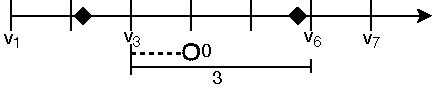
\includegraphics[width=0.7\linewidth]{img/problem.pdf}
%	\caption{Example change history of query $q_1$.}
%	\label{fig:problem}
%\end{figure}

\paragraph{Architecture:} In Figure~\ref{fig:schema}, we provide an overview of our proposed architecture for making predictions with respect to the OSC and TTL tasks. A SPARQL query $Q$ and a dynamic RDF graph $\mathcal{G}$ are given as input. The first component parses the query and generates static features which include statistics about the number of elements in the query (e.g., number of triple patterns, variables, etc.) as well as the presence of particular query operators (e.g., \texttt{UNION}, \texttt{FILTER}, recursive path expressions, etc.). The second component may take as input some features of the query, as well as information from the dynamic graph, and produce a set of further features; this component may compute, for example, statistics about the dynamicity of predicates used in the query, or statistics about changes in the query results over past versions. The final features are passed to a classifier in the case of the OSC problem, and to a regression model in the case of the TTL problem, to generate the final output prediction. We will now describe in more detail the query and data features considered in this work.

%\begin{figure*}[!t]
%	\centering
%	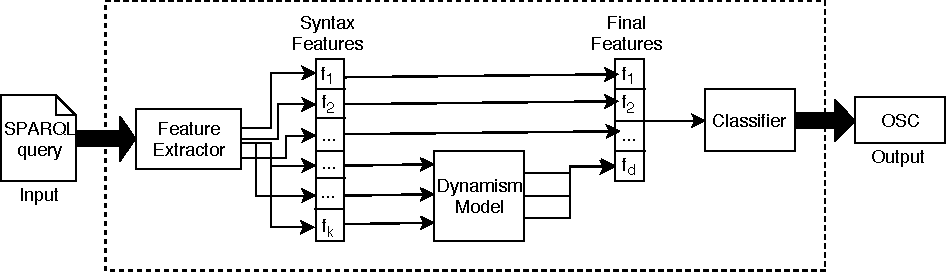
\includegraphics[width=0.9\linewidth]{img/schema.pdf}
%	\caption{Proposed architecture with Feature Extractor and Dynamics Model \ah{What is $g$ here and why is it output from the Dynamics Model (rather than input)?}}
%	\label{fig:schema}
%\end{figure*}

\begin{figure}[tb]
\newlength{\hgap}
\setlength{\hgap}{0.7cm}

\newcommand{\tb}[1]{\begin{tabular}{c} #1 \end{tabular}}
\newcommand{\hsp}{\vphantom{Ag}}

\tikzset{
    every node/.style={
    	font=\sffamily,
    },
	f/.style={ 
		draw,
		text centered,
		style={inner sep=0.8},
		font=\footnotesize,
		minimum width=1.3em,
		minimum height=1.2em
	},
	i/.style={ 
		draw,
		text centered,
		rounded corners
	},
	o/.style={ 
		draw,
		text centered,
		rounded corners
	},	
	c/.style={ 
		draw,
		top color=white, 
		bottom color=black!5
	},	
	arrout/.style={
		->,
		-latex,
		black!25},
	arrin/.style={
        <-,
        latex-,
		black!25},	
}

\centering
\resizebox{0.9\textwidth}{!}{
\begin{tikzpicture}
\node[i] (q) {$Q$};

\node[c,right=\hgap of q] (qfe) {\tb{Query \\ Feature \\ Extractor}}
  edge[arrin] (q);

\node[f,right=1.5\hgap of qfe] (f4) {\tiny ...};
\node[f,anchor=south] (f3) at (f4.north) {\tiny ...};
\node[f,anchor=south] (f2) at (f3.north) {\tiny ...};
\node[f,anchor=south] (f1) at (f2.north) {$f_1$};
\node[f,anchor=north] (f5) at (f4.south) {\tiny ...};
\node[f,anchor=north] (f6) at (f5.south) {\tiny ...};
\node[f,anchor=north] (fn) at (f6.south) {$f_n$};  

\draw [arrout] (qfe.east) -- + (0.3,0) |- (f1);
\draw [arrout] (qfe.east) -- + (0.3,0) |- (f2);
\draw [arrout] (qfe.east) -- + (0.3,0) |- (f3);
\draw [arrout] (qfe.east) -- + (0.3,0) |- (f4);
\draw [arrout] (qfe.east) -- + (0.3,0) |- (f5);
\draw [arrout] (qfe.east) -- + (0.3,0) |- (f6);
\draw [arrout] (qfe.east) -- + (0.3,0) |- (fn);
  
\node[c,right=\hgap of fn] (dfe) {\tb{Data\\Feature\\Extractor}}
  edge[arrin] (fn); 
  
\draw[arrout] (f6.east) -- (dfe.west|-f6.east);
  
\node[i,anchor=south] (g) at (q.mid|-dfe.south) {$\mathcal{G}$}
  edge[arrout] (dfe.west|-g.east);  
  
\node[f,right=\hgap of dfe] (dfk) {$f'_k$}
  edge[arrin] (dfe);    
\node[f,anchor=south] (df6) at (dfk.north) {\tiny ...}
  edge[arrin] (dfe.east|-df6);  
\node[f,anchor=south] (df5) at (df6.north) {$f_j$}
  edge[arrin] (f5);    
\node[f,anchor=south] (df4) at (df5.north) {\tiny ...}
  edge[arrin] (f4);  
\node[f,anchor=south] (df3) at (df4.north) {\tiny ...}
  edge[arrin] (f3);      
\node[f,anchor=south] (df2) at (df3.north) {\tiny ...}
  edge[arrin] (f2);   
\node[f,anchor=south] (df1) at (df2.north) {$f_1$}
  edge[arrin] (f1);  
  
\node[c,right=1.5\hgap of df2,minimum width=6.5em] (c) {Classification\hsp};

\draw [arrout] (df1.east) -- + (0.3,0) |- (c);
\draw [arrout] (df2.east) -- + (0.3,0) |- (c);
\draw [arrout] (df3.east) -- + (0.3,0) |- (c);
\draw [arrout] (df4.east) -- + (0.3,0) |- (c);
\draw [arrout] (df5.east) -- + (0.3,0) |- (c);
\draw [arrout] (df6.east) -- + (0.3,0) |- (c);
\draw [arrout] (dfk.east) -- + (0.3,0) |- (c);

\node[c,right=1.5\hgap of df6,minimum width=6.5em] (r) {Regression\hsp};

\draw [arrout] (df1.east) -- + (0.3,0) |- (r);
\draw [arrout] (df2.east) -- + (0.3,0) |- (r);
\draw [arrout] (df3.east) -- + (0.3,0) |- (r);
\draw [arrout] (df4.east) -- + (0.3,0) |- (r);
\draw [arrout] (df5.east) -- + (0.3,0) |- (r);
\draw [arrout] (df6.east) -- + (0.3,0) |- (r);
\draw [arrout] (dfk.east) -- + (0.3,0) |- (r);

\node[o,right=\hgap of c] (osc) {\tb{OSC \\ Prediction}}
  edge[arrin] (c);
  
\node[o,right=\hgap of r] (ttl) {\tb{TTL \\ Prediction}}
  edge[arrin] (r);    

\end{tikzpicture}
}

\caption{Proposed architecture for predicting change in query results\label{fig:schema}}
\end{figure}

\paragraph{Query Features:} Our initial set of features are based on analysis of the input SPARQL query. Figure~\ref{fig:query} shows only a sample of the evaluated features, as well as -- for the purposes of illustration -- their values for an accompanying example query. 

The first block of features capture statistics about the query, indicating loosely its size and complexity. One may consider that the higher these values are, in general, the more dynamic we can expect the query to be since there are more ``opportunities'' for the query results to be affected by change. In some cases, however, the hypothesized correlation is not direct since, for example, adding more triple patterns may serve to narrow the query down and focus it on a static part of the graph (e.g., when looking for the movies of directors, adding a triple pattern to restrict the results to directors who have died). Hence it will be of interest to see how these features affect the predictions made experimentally.

The second block indicate the query operators used; we capture the presence or absence of query operators and solution modifiers from SPARQL 1.1. In the third block, we group related features into one dimension: in the case of \textit{Recursive path}, we group queries that contain as expression of the form $e$\texttt{*} or $e$\texttt{+}. On the other hand, in \textit{Negation}, we group non-monotonic features that allow for modeling difference (\texttt{MINUS}, \texttt{NOT EXISTS}, \texttt{!BOUND}). These features -- though course-grained -- are straightforward to extract from a query, and offer valuable insights into how the query may behave in a dynamic query; for example, the \textit{Negation} feature captures information about the (non-)monotonicity of the query, while we suppose that \textit{Recursive paths}, which may traverse an arbitrary number of triples in the graph, might be more sensitive to change. Again, such correlations are not without exception and will require experimental scrutiny.

The final feature is the set of all predicates used in a triple pattern, including (where applicable) the IRIs used in a path expression; this is rather a meta-feature that serves as input for the next part of the proposed model.

\begin{figure}[!t]
{\centering
	\begin{minipage}{0.46\textwidth}
	\begin{lstlisting}[style=sparqld]
SELECT ?item
WHERE {
  ?item :instance_of :human .
  ?item :gender :female .
    { ?item :place_of_birth :Wales }
  UNION
    { ?item :place_of_birth ?pob .
      ?pob :located_in* :Wales }
  OPTIONAL 
    { ?sitelink schema:about ?item .
      ?sitelink schema:inLanguage "cy" }
  FILTER (!BOUND(?sitelink))
}
LIMIT 100
	\end{lstlisting}
	\end{minipage}}
	\hfill
	\resizebox{0.45\textwidth}{!}{
	\begin{tabular}{lr}    \toprule
		\ntextnumero of triple patterns        & 7			\\
		\ntextnumero of variables      & 3			\\
		\ntextnumero of projected variables & 1			\\
		\ntextnumero of predicates     & 6			\\ \midrule
		\texttt{FILTER}            	& \tickYes	\\
		\texttt{LIMIT}             	& \tickYes	\\
		\texttt{UNION}             	& \tickYes	\\
		\texttt{GROUPBY}     & \tickNo			\\ \midrule 
		\textit{Sub-query}         	& \tickNo	\\
		\textit{Recursive path}		& \tickYes	\\
		\textit{Negation}         		& \tickYes	\\ \midrule
		\textit{Predicates}			& $\{$ \texttt{:instance\_of}, ... $\}$     \\    \bottomrule
	\end{tabular}	
	}
\caption{Example query and a sample of the features extracted from it \label{fig:query}}	
\end{figure}

\paragraph{Data Features (predicate dynamics):} The next component in our architecture can extract features that capture information about the query \textit{and} the dynamic graph under consideration.  The first such feature we consider captures how many triples change for a predicate in a time interval, with the idea that -- as in previous works~\cite{UmbrichKHP12,UmbrichKPPH12,ekawUmbrichKHP12,DehghanzadehPKUHD14} -- predicates capture rich information about the dynamics of a dataset, where the results of queries with dynamic predicates will be more sensitive to change; furthermore, given that in most datasets the number of predicates is relatively low (in the thousands or tens of thousand), such statistics are quite lightweight to maintain and compute. Formally, given two RDF graphs $G_i$ and $G_j$, we denote by $G_i \oplus G_j$ the set of triples $(G_i \cup G_j) - (G_i \cap G_j)$ where ``$-$'' denotes set difference; in other words, $G_i \oplus G_j$ denotes the triples in one graph or the other but not both (noting that $G_i \oplus G_j = G_j \oplus G_i$). Next, given an RDF graph $G$ and an IRI $p$, let $\#(G,p) \da |\{(x,y,z) \in G : y = p \}|$ denote the number of triples in $G$ with predicate $p$. Finally, given a dynamic RDF graph $\mathcal{G} \da ( G_1, \ldots, G_n )$ and a predicate $p$, we denote by $\Delta(\mathcal{G},p) \da \Sigma_{i=1}^{n-1}\frac{\#(G_i \oplus G_{i+1},p)}{\#(G_i \cup G_{i+1},p)}$ the normalized sum of the number of triples with the predicate $p$ that changed between pairs of consecutive versions.

%\begin{definition}[Predicate Multiplicity of an RDF Dataset]
%	Given an RDF dataset $d$ and a predicate $p$, the multiplicity of $p$ in $d$, denoted by $M(p,d)$, is:
%	\begin{equation}
%	\label{eq:pm}
%	M(p,d) = |\{(x,y,z) \in d : y = p \}|
%	\end{equation}
%\end{definition}
%
%
%\begin{example}
%	\label{ex:pm}    
%	Considering Example~\ref{ex:dataset}, the Predicate Multiplicity of predicate \textit{image} in $d_6$ dataset is:    $M(image,d_6) = 2$
%\end{example}
%
%Then, we must capture the change between two versions of an RDF dataset at the triples level, which represents triples added and deleted between the versions. For this purpose, we define a \textit{Difference Set} as an RDF dataset denoted by $\Delta(d_1, d_2)$ applying low-level change detection techniques.
%
%\begin{definition}[Difference Set]
%	Let $d_1$ and $d_2$ be two RDF datasets; a Difference Set denoted by $\Delta(d_1, d_2)$ is:
%	\begin{equation}
%	\label{eq:ds}
%	\Delta(d_1, d_2) = \{t \mid t \in d_2 \wedge t \notin d_1\} \cup \{t \mid t \in d_1 \wedge t \notin d_2\}
%	\end{equation}
%\end{definition}
%
%\begin{example}
%	\label{ex:ds}
%	We show the Difference Set between versions $d_1$ and $d_6$:\\
%	\begin{center}    
%		\begin{tabular}{lll}    \hline
%			\multicolumn{3}{c}{$\Delta(d_1, d_6)$} \\    \hline
%			-    :Atlantic\_Ocean  & :temperature   & 40$\degree$F          \\
%			+    :Atlantic\_Ocean  & :temperature   & 60$\degree$F          \\
%			+    :Atlantic\_Ocean  & :image         & AOcean2.png              \\    \hline
%		\end{tabular}
%	\end{center}
%	
%	We can now denote the Predicate Multiplicity of a Difference Set of $d_1$ and $d_2$ by $M(p, \Delta(d_1, d_2))$, e.g., $M(image, \Delta(d_1, d_6)) = 1$.
%\end{example}
%
%
%Following the intuition of our model, we now look for the multiplicity of a predicate $p$ of a dynamic dataset $\mathcal{D}$ in a time interval $[n,m]$.
%
%\begin{definition}[Aggregated Predicate Multiplicity of a dynamic dataset]
%	Let $\mathcal{D} = (d_1, d_2, ..., d_m)$ be a dynamic dataset, and $p$ a predicate. The Aggregated Predicate Multiplicity of $\mathcal{D}$ in a time interval $[n,m]$, denoted by $AM(p, \mathcal{D},[n,m])$ is:
%	\begin{equation}
%	\label{eq:apm}
%	AM(p, \mathcal{D},[n,m]) = \sum_{i=n}^{m-1}M(p, \Delta(d_i, d_{i+1}))
%	\end{equation}
%\end{definition}
%
%\begin{example}
%	\label{ex:apm}
%	$AM(temperature, \mathcal{D},[1, 7]) =$
%	
%	$ \sum_{i=1}^{6}M(temperature, \Delta(d_i, d_{i+1})) = 4$
%	
%	\begin{center}    
%		\begin{tabular}{lll}    \hline
%			\multicolumn{3}{c}{$\sum_{i=1}^{6}\Delta(d_i, d_{i+1})$} \\    \hline
%			-    :Atlantic\_Ocean  & :temperature   & 40$\degree$F          \\
%			+    :Atlantic\_Ocean  & :temperature   & 50$\degree$F          \\            
%			-    :Atlantic\_Ocean  & :temperature   & 50$\degree$F          \\
%			+    :Atlantic\_Ocean  & :temperature   & 60$\degree$F          \\
%			+    :Atlantic\_Ocean  & :image         & AOcean2.png              \\    \hline
%		\end{tabular}
%	\end{center}
%\end{example}
%
%We can now denote the Aggregated Multiplicity of a dynamic dataset in a time interval $[n,m]$ by:
%
%\begin{equation}
%\label{eq:am}
%AM(\mathcal{D},[n,m]) = \sum_{p \in P}AM(p, \mathcal{D},[n,m])
%\end{equation}\\
%Where $ P $ denotes the set of all predicates that have changed in the interval $[n,m]$.
%
%\begin{example}
%	\label{ex:am}
%	$AM(\mathcal{D},[1,7]) = AM(temperature, \mathcal{D},[1,7])$
%	
%	$+ AM(image, \mathcal{D},[1,7]) = 5$
%\end{example}
%
%Finally, the \textit{Dynamics} of a predicate is given by the \textit{Aggregated Predicate Multiplicity of a dynamic dataset} $\mathcal{D}$ divided by \textit{Aggregated Multiplicity of a dynamic dataset}.
%
%\begin{equation}
%\label{eq:dyn}
%Dyn(p, \mathcal{D},[n,m]) = \frac{AM(p, \mathcal{D},[n,m])}{AM(\mathcal{D},[n,m])}
%\end{equation}
%
%\begin{example}
%	\label{ex:dyn}
%	Considering our example:
%	
%	$ Dyn(temperature, \mathcal{D},[1,7]) = \frac{4}{5} = 0.8$
%	
%	$ Dyn(image, \mathcal{D},[1,7]) = \frac{1}{5} = 0.2$
%	
%	$ Dyn(area, \mathcal{D},[1,7]) = \frac{0}{5} = 0$
%\end{example}
%
%Considering our proposed model, the Dynamics Model component receives the set of predicates extracted from the queries, calculates the $Dyn(p, \mathcal{D},[n,m])$ for each predicate $p$ and provides the value of a Transformation Function on these indicators. The intention of the Transformation Function is to estimate the dynamics of the query based on the Dynamics of the predicates.

\begin{figure}[!t]
{\centering
	\begin{minipage}{0.32\textwidth}
	\begin{lstlisting}[style=sparqld]
:LMessi :name "L. Messi" ;
 :instance_of :Human ;
 :children 1 ;
 :played :2014WC .
	\end{lstlisting}
	\end{minipage}	
\hfill
\begin{minipage}{0.32\textwidth}
	\begin{lstlisting}[style=sparqld]
:LMessi :name "L. Messi" ;
 :children 2 ;
 :played :2014WC, :2018WC .
	\end{lstlisting}
\end{minipage}	
\hfill
\begin{minipage}{0.32\textwidth}
	\begin{lstlisting}[style=sparqld]
:LMessi :name "L. Messi" ;
 :instance_of :Human ;
 :children 3 ;
 :played :2014WC, :2018WC .
	\end{lstlisting}
\end{minipage}	
}

\caption{Example dynamic RDF graph $\mathcal{G} = (G_1, G_2, G_3)$ (from left to right, resp.) \label{fig:dg}}
\end{figure}

\begin{figure}[!t]
{\centering
\hfill
	\begin{minipage}{0.35\textwidth}
	\begin{lstlisting}[style=sparqld]
:LMessi :instance_of :Human ;
 :children 1 , 2 ;
 :played :2014WC .
	\end{lstlisting}
	\end{minipage}	
\hfill
\begin{minipage}{0.35\textwidth}
	\begin{lstlisting}[style=sparqld]
:LMessi :instance_of :Human ;
 :children 2 , 3 .
	\end{lstlisting}
\end{minipage}	
\hfill
}
\caption{Changes for $\mathcal{G}$ in Figure~\ref{fig:dgc}, showing $G_1 \oplus G_2$ (left) and $G_2 \oplus G_3$ (right) \label{fig:dgc}}
\end{figure}

\begin{example}
Consider the example dynamic RDF graph $\mathcal{G}$ in Figure~\ref{fig:dg} (based on real data from Wikidata, with IRIs modified for the purposes of readability). In Figure~\ref{fig:dgc} we show the pairwise changes between each version: $G_1 \oplus G_2$ and $G_3 \oplus G_4$. For a predicate $p$, the value $\Delta(\mathcal{G},p)$ is then the sum of triples with predicate $p$ in the graphs $G_1 \oplus G_2$ and $G_2 \oplus G_3$ divided by the number of triples with predicate $p$ in the graphs $G_1 \cup G_2$ and $G_2 \cup G_3$. Looking at Figure~\ref{fig:dgc}, for example, \texttt{:name} does not appear ($\Delta(\mathcal{G},\texttt{:name})=0$), \texttt{:children} appears twice in $G_1 \oplus G_2$ and $G_1 \cup G_2$, as well as, twice in $G_2 \oplus G_3$ and $G_2 \cup G_3$ ($\Delta(\mathcal{G},\texttt{:children})=4/4=1$), and so forth.
\end{example}

Given a query $Q$ with a set of predicates $\{ p_i, ..., p_n \}$, we may then consider a variety of aggregate functions over $\Delta(\mathcal{G},p_1), ..., \Delta(\mathcal{G},p_n)$, such as $\mathrm{max}$, $\mathrm{mean}$, etc., to compute a final numeric feature for the query, representing a summary of the level of dynamicity of the predicates it contains.

\paragraph{Data Features (result dynamics):} The second data feature we capture indicates how many times the query results $Q$ have changed over the past versions of the dynamic graph. While this feature offers rich information for prediction, given a query that has not previously been seen, it is costly to compute, since it requires the execution of the query over each past version within an interval, which in turn requires maintaining indexes over a variety of past versions.

\section{Gold Standard Dataset}
\label{sec:data}

In order to evaluate the effectiveness of our proposal for predicting changes in SPARQL query results, we require a dynamic RDF graph, with access to various historical versions; preferably this graph contains real-world, large-scale, diverse data, and with sufficient changes between versions to provide both positive and negative examples of queries whose results change. Furthermore, we require a set of SPARQL queries that can be answered against this dynamic graph; preferably these queries again should be diverse, representative of real-world user queries, of a variety of shapes and sizes, using a variety of query operators, and with a mix of both dynamic and static results over the dynamic graph. In particular, we choose Wikidata~\cite{VrandecicK14} for our experiments, which, we shall argue, meets the aforementioned requirements. We first give details of the dynamic data we collect from Wikidata; thereafter, we discuss the queries we use in our experiments.

\paragraph{RDF Data:} We use 23 Wikidata snapshots from 18/04/2017 to 27/09/2017, which are captured almost weekly($\pm$ 1 day) in the \emph{truthy version} that contains triples (without qualifiers) that have the best non-deprecated rank for a given property. The first version has 1,102,242,331 triples and 3,276 unique predicates, while the final version has 1,924,967,162 triples (+74\%) and 3,660 unique predicates (+11\%). Figure~\ref{fig:wikidata}, on the left, shows the growth in triples as the time progress, while on the right, shows the numbers of triples added and removed version-to-version. We see that although many more triples are added than removed, there are some triples removed each version. We further note some peaks in triples added in some versions, which may be due to bulk imports of data. Between the version 11 and 12 we have almost 2 weeks because we were not able to obtain the data for that week, but this cause the third highest peak. The dynamic graph thus considers a total of 32.3 billion triples across 23 versions.

\begin{figure}[t]
	%\begin{minipage}[b]{0.47\linewidth}
		\centering
		\begin{tikzpicture}[thick,font=\scriptsize]
		\begin{axis}[
		%title={Temperature dependence of CuSO$_4\cdot$5H$_2$O solubility},
		xlabel={Version},
		width=5cm, 
		height=5cm,
		ymin=0,
		xtick={1,2,...,23},
		xticklabels={},
		extra x ticks={1,23},
		legend pos=north west,
		ymajorgrids=true,
		grid style=dashed,
		]
		
		\addplot[
		color=blue,
		mark=diamond,
		]
		coordinates {
			(1,1102242331)(2,1138975810)(3,1141303957)(4,1170283653)(5,1176093821)(6,1184177503)(7,1190456714)(8,1211813217)(9,1239145151)(10,1271353260)(11,1293099057)(12,1348622441)(13,1418460320)(14,1432143355)(15,1470298276)(16,1506140622)(17,1542278452)(18,1593334993)(19,1613832004)(20,1684774955)(21,1771601730)(22,1843086909)(23,1924967162)
		};
		
		%\legend{# entities}
		%\legend{# predicates}
		%\legend{# literals}
		%\legend{# blank nodes}
		
		\end{axis}
		\end{tikzpicture}
%		\caption{Evolution of the number of triples on Wikidata.}
%		\label{graph:datasize}
%	\end{minipage}
	\hspace{0.1cm}
%	\begin{minipage}[b]{0.47\linewidth}
%		\centering
		\begin{tikzpicture}[thick,font=\scriptsize]
		\begin{axis}[
		xlabel={Version},
		x tick label style={
			/pgf/number format/1000 sep=},
		%ylabel=\#Triples,
		width=9cm, 
		height=5cm,
		enlarge x limits=0.04,
		enlarge y limits=0,
		ymax=80000000,
		legend style={at={(0.25,0.95)},
			anchor=north,legend columns=-1},
		ybar=0pt,
		xtick=data,
		xtick align=inside,
		bar width=3pt,
		ymajorgrids,
		grid style=dashed,
		]
		\addplot 
		coordinates {(1,40137188)(2,4563382)(3,29302968)(4,8906402)(5,11455047)(6,11435682)(7,27229516)(8,26968577)(9,38952400)(10,20283316)(11,49001368)(12,70073220)(13,17685830)(14,45405782)(15,41199256)(16,42633484)(17,56683899)(18,25309217)(19,25030143)(20,22548371)(21,23330356)(22,37009794)};
		\addplot 
		coordinates {(1,3403743)(2,2235268)(3,1116111)(4,3096270)(5,3371448)(6,5156519)(7,5873153)(8,1336452)(9,6744349)(10,999601)(11,786939)(12,1123311)(13,4002828)(14,7250907)(15,5356971)(16,6495717)(17,5627376)(18,4812243)(19,790590)(20,681118)(21,1194899)(22,998105)};
		\legend{Added, Removed}
		\end{axis}
		\end{tikzpicture}
\caption{Evolution of total triples in Wikidata (left) and number of triples added to and removed from the $n$\textsuperscript{th} version for the $n+1$\textsuperscript{th} version (right) \label{fig:wikidata}}
\end{figure}

Although we have seen that the number of unique predicates did not change much over all versions, we are interested to see which predicates are indicative of dynamic statements. Table~\ref{tab:predicates} shows the ten most dynamic predicates according to the number statements involving that predicate (left) and the ratio of added (+) and deleted (−) statements divided by the total number of statements for that predicate across all snapshots; for the second, we only include predicates that appear in all snapshots and appear in ≥ 1, 000 statements overall. Note that the largest number of changes involves the predicate scheme:description, however, its dynamic value is low due to the number of statements with it in the versions.  

\begin{figure}[!t]
	\caption{Top-10 dynamic predicates according with total (left) and proportional (right) changes}
	\label{tab:predicates}
	\resizebox{0.45\textwidth}{!}{
		\begin{tabular}{rlrr}    \toprule
			\ntextnumero        & Predicate & Total	& Dyn 	\\  \midrule
			1 & schema:description  & 464567354  	& 0.04   \\
			2 & schema:dateModified  & 99330382  	& 0.14   \\
			3 & schema:version  & 99330164  	& 0.14  \\
			4 & schema:name  & 44487864  	& 0.01   \\
			5 & rdfs:label  & 44487864  	& 0.01   \\
			6 & skos:prefLabel  & 44487864  	& 0.01   \\
			7 & wdt:P2093(author name)  & 30671685  	& 0.09   \\
			8 & rdf:type  & 21808957  	& 0.02   \\
			9 & wdt:P31(instance of)  & 12483471  	& 0.02   \\
			10 & schema:about  & 10773295  	& 0.02  \\    \bottomrule
		\end{tabular}	
	}
	\hfill
	\resizebox{0.5\textwidth}{!}{
		\begin{tabular}{rlrr}    \toprule
			\ntextnumero        & Predicate & Total	& Dyn 	\\  \midrule
			1 & owl:complementOf & 156862 & 0.99	\\
			2 & owl:onProperty & 156862 & 0.99	\\
			3 & owl:someValuesFrom & 86674 & 0.71	\\
			4 & wdt:P2462(member of the deme) & 3563 & 0.62	\\
			5 & wdt:P3383(film poster) & 4388 & 0.58	\\
			6 & wdt:P2331(Cycling Archives ID) & 4229 & 0.33	\\
			7 & wdt:P1112() & 4366 & 0.20	\\
			8 & wdt:P505(general manager) & 4959 & 0.18	\\
			9 & schema:dateModified & 99330382 & 0.14	\\
			10 & schema:version & 99330164 & 0.14	\\    \bottomrule
		\end{tabular}	
	}	
\end{figure}

%\subsection{Queries Dataset}

\paragraph{Queries:} In order to achieve a set of SPARQL queries that are answerable over Wikidata and with which we could run experiments, we took the user-contributed example queries from the Wikidata Query Service\footnote{https://www.wikidata.org/wiki/Wikidata:SPARQL\_query\_service/queries/examples}, consisting of 389 SPARQL 1.1 \texttt{SELECT} queries of varying degrees of complexity, touching upon various domains of data, and with a mix of varying query operators.\footnote{Very recently, a large log of millions of SPARQL queries have been released for Wikidata~\cite{MalyshevKGGB18}; these queries were not available when conducting our experiments, but would be interesting to analyze as part of future work.}

96 queries had to be removed from the original set of 389 because they asked for information external to Wikidata (using \texttt{SERVICE}) or asked for qualifiers that are not present in the truthy version. We also eliminated 12 queries that returned bindings to blank nodes to facilitate comparison between the results. Furthermore, some queries featured non-deterministic elements -- such as \texttt{LIMIT}/\texttt{OFFSET} without ordering, \texttt{SAMPLE} or temporal functions -- such as \texttt{TODAY()} -- that may lead to changes in results not related to changes in the data; we remove 23 queries with \texttt{SAMPLE} and temporal functions, and add an \texttt{ORDER BY} clause to all queries to ensure determinism with \texttt{LIMIT}/\texttt{OFFSET} and more generally to facilitate quick comparison of results. We also eliminated 37 queries with 0 results in the executions over all the snapshots. As a result of this process of filtering, we end up with a total of 221 deterministic queries.

Furthermore, we needed to transform certain queries for the purposes of our experiments. 163 queries used features particular to the Wikidata Query Service, such as using a custom label \texttt{SERVICE} call to specify language preferences; we converted these queries to standard SPARQL using \texttt{COALESCE} to capture preferences.  Figure~\ref{fig:transform} shows an example of a Wikidata query with the \texttt{LABEL} service rewritten and a deterministic ordering added. 

\begin{figure}[!t]
\centering
{
	\begin{minipage}{0.8\textwidth}
	\begin{lstlisting}[style=sparqld]
#Cats
SELECT ?item ?itemLabel
WHERE {
 ?item wdt:P31 wd:Q146 .
 SERVICE wikibase:label { bd:serviceParam wikibase:language "en,es" }
}
	\end{lstlisting}
	\end{minipage}	
}

{
\begin{minipage}{0.8\textwidth}
	\begin{lstlisting}[style=sparqld]
#Cats
SELECT ?item ?itemLabel
WHERE {
  ?item wdt:P31 wd:Q146 .
  OPTIONAL { ?item rdfs:label ?en . FILTER(lang(?en)="en") }
  OPTIONAL { ?item rdfs:label ?es . FILTER(lang(?es)="es") }
  BIND(str(coalesce(?en, ?es, strafter(str(?item),
    "http://www.wikidata.org/entity/"))) AS ?itemLabel )
}
ORDER BY ?item ?itemLabel
	\end{lstlisting}
\end{minipage}	
}
\caption{Query transformation before (above) and after (below) \label{fig:transform}}
\end{figure}

In Table~\ref{tab:Pattern}, we provide statistics on the distribution of different types of triple patterns in the 221 queries before the transformation; of key importance is that 86.20\% of the triple patterns have a constant in the predicate position, meaning that they are compatible with a model based on the dynamics of predicates. We also see that 83 triple patterns (11.34\%) feature a path expression, where Table~\ref{tab:Path} provides the distribution of these expressions (remarking that multiple patterns can be used in one expression); of note here is that recursion is commonly found (74.70\% use $e\texttt{*}$ while 9.64\% use $e\texttt{+}$), and that we find no negated property paths.

\begin{table}[t]
	\begin{minipage}[b]{0.47\linewidth}
		\centering
		\caption{Distribution of triple patterns (C: Constant, V: Variable, P: Path). \label{tab:Pattern}}
		\begin{tabular}{lrr}    \toprule
			\textbf{Pattern} & \textbf{\ntextnumero} & \textbf{\%} \\    \midrule
			V C V   & 435      & 59.43\%    \\
			V C C   & 190      & 25.96\%    \\
			V V V   & 9        & 1.23\%     \\
			C C V   & 6        & 0.82\%     \\
			V V C   & 5        & 0.68\%     \\
			C V V   & 3        & 0.41\%     \\
			C V C   & 1        & 0.14\%     \\
			C C C   & 0        & 0.00\%     \\    \midrule
			V P C   & 69       & 9.43\%     \\
			V P V   & 13       & 1.78\%     \\
			C P V   & 1        & 0.14\%     \\
			C P C   & 0        & 0.00\%     \\    \bottomrule
		\end{tabular}
	\end{minipage}
	\hfill
	\begin{minipage}[b]{0.47\linewidth}
		\centering
		\caption{Distribution of paths\label{tab:Path}}
		\begin{tabular}{lrr}    \toprule
			\textbf{Pattern}      & \textbf{\ntextnumero} & \textbf{\%} \\    \midrule
			$e\texttt{*}$   & 62       & 74.70\%     \\
			$e_1 \texttt{/} e_2$  & 56       & 67.47\%    \\
			$e\texttt{+} $   & 8        & 9.64\%     \\
			$e_1 \texttt{|} e_2$  & 6        & 7.23\%     \\
			$e\texttt{?}$    & 6        & 7.23\%     \\
			$\texttt{!(}e\texttt{)}$ & 0        & 0.00\%        \\ \midrule
			$e$ & 83 & 100.00\% \\
			\bottomrule
		%	$P \rightarrow C $    & 83       & 100.00\%      \\    \bottomrule
		\end{tabular}
	\end{minipage}
\end{table}

Finally, we look at how the results for these queries change over the 23 versions. Figure~\ref{graph:changeV} shows how many queries had some results change between two consecutive versions, where we see that approximately half of the queries see changes in their results each version. But are these always the same queries that change every time? Figure~\ref{graph:changeV} shows the number of versions in which some result changed for each query; the queries are ordered by the number of changes in their results, where we can see that the results of 44 queries (19.90\%) change each time, 17 queries (7.69\%) never change, and more generally, we note a quite uniform distribution of queries in between. More generally speaking, we conclude that our query set has a good balance of queries whose results never change, queries whose results always change, and queries whose results sometimes change.

\begin{figure}[t]
	\begin{minipage}[b]{0.47\linewidth}
		\centering
		\begin{tikzpicture}[thick,font=\scriptsize]
		\begin{axis}[
		xlabel={Version},
		ylabel={Queries changed},
		ylabel near ticks,
		width=6.5cm, 
		height=5cm,
		ymin=0, ymax=221,
		xtick={1,2,...,23},
		xticklabels={},
		extra x ticks={1,23},
		legend pos=north west,
		ymajorgrids=true,
		grid style=dashed,
		]
		
		\addplot[
		color=blue,
		mark=diamond,
		]
		coordinates {
			(1,115)(2,112)(3,118)(4,116)(5,121)(6,111)(7,127)(8,109)(9,118)(10,115)(11,129)(12,105)(13,113)(14,118)(15,117)(16,111)(17,118)(18,112)(19,116)(20,106)(21,106)(22,129)
		};
		
		%\legend{# entities}
		%\legend{# predicates}
		%\legend{# literals}
		%\legend{# blank nodes}
		
		\end{axis}
		\end{tikzpicture}
		\caption{Number of queries with some results changed for each version}
		\label{graph:changeV}
	\end{minipage}
	\hspace{0.7cm}
	\begin{minipage}[b]{0.47\linewidth}
		\centering
		\begin{tikzpicture}[thick,font=\scriptsize]
		\begin{axis}[
		xlabel={Query},
		ylabel={Versions changed},
		ylabel near ticks,
		width=6.5cm, 
		height=5cm,
		ymin=0,
		legend pos=north west,
		ymajorgrids=true,
		grid style=dashed,
		]
		
		\addplot[
		color=blue
		]
		coordinates {
			(1,22)(2,22)(3,22)(4,22)(5,22)(6,22)(7,22)(8,22)(9,22)(10,22)(11,22)(12,22)(13,22)(14,22)(15,22)(16,22)(17,22)(18,22)(19,22)(20,22)(21,22)(22,22)(23,22)(24,22)(25,22)(26,22)(27,22)(28,22)(29,22)(30,22)(31,22)(32,22)(33,22)(34,22)(35,22)(36,22)(37,22)(38,22)(39,22)(40,22)(41,22)(42,22)(43,22)(44,22)(45,21)(46,21)(47,21)(48,21)(49,21)(50,21)(51,21)(52,20)(53,20)(54,20)(55,20)(56,20)(57,20)(58,20)(59,20)(60,19)(61,19)(62,19)(63,19)(64,19)(65,19)(66,18)(67,18)(68,18)(69,18)(70,18)(71,18)(72,18)(73,18)(74,17)(75,17)(76,17)(77,17)(78,16)(79,16)(80,16)(81,16)(82,16)(83,16)(84,15)(85,15)(86,15)(87,15)(88,15)(89,15)(90,15)(91,15)(92,14)(93,14)(94,14)(95,14)(96,13)(97,13)(98,13)(99,13)(100,13)(101,13)(102,13)(103,13)(104,12)(105,12)(106,12)(107,12)(108,12)(109,12)(110,11)(111,11)(112,11)(113,11)(114,11)(115,11)(116,11)(117,11)(118,10)(119,10)(120,10)(121,10)(122,10)(123,10)(124,10)(125,9)(126,9)(127,9)(128,9)(129,9)(130,9)(131,8)(132,8)(133,8)(134,8)(135,8)(136,7)(137,7)(138,7)(139,7)(140,7)(141,7)(142,7)(143,7)(144,6)(145,6)(146,6)(147,6)(148,6)(149,6)(150,6)(151,6)(152,5)(153,5)(154,5)(155,5)(156,5)(157,5)(158,4)(159,4)(160,4)(161,4)(162,4)(163,4)(164,4)(165,4)(166,4)(167,4)(168,4)(169,3)(170,3)(171,3)(172,3)(173,3)(174,3)(175,2)(176,2)(177,2)(178,2)(179,2)(180,2)(181,2)(182,2)(183,2)(184,2)(185,2)(186,2)(187,2)(188,2)(189,2)(190,1)(191,1)(192,1)(193,1)(194,1)(195,1)(196,1)(197,1)(198,1)(199,1)(200,1)(201,1)(202,1)(203,1)(204,1)(205,0)(206,0)(207,0)(208,0)(209,0)(210,0)(211,0)(212,0)(213,0)(214,0)(215,0)(216,0)(217,0)(218,0)(219,0)(220,0)(221,0)
		};
		
		%\legend{# entities}
		%\legend{# predicates}
		%\legend{# literals}
		%\legend{# blank nodes}
		
		\end{axis}
		\end{tikzpicture}
		\caption{Number of versions in which some results changed for each query}
		\label{graph:changeH}
	\end{minipage}
\end{figure}

\paragraph{Feature extraction:} To compute the query features, we use Apache Jena to parse the query and extract the necessary statistics and determine the presence of the relevant query operators. In order to extract statistics on the dynamics of individual predicates in the dynamic graph, a challenge here is scalability, since we work with a total of 32.3 billion triples; hence we (1) sort each version of Wikidata, (2) apply a merge-sort iterator over each pair of consecutive versions ($G_i$ and $G_{i+1}$) to detect triples that changed ($G_i \oplus G_j$), writing a separate file for triples that were deleted ($G_i - G_j$) and added ($G_j - G_i$), (3) from these files, we can then compute and sum the number of triples changed for each predicate between each pair of versions. Finally, in order to create the ground truth in terms of which results change between which versions, we index each version in Virtuoso and compute the results for each query against each version and write them to disk; we then compare consecutive pairs of results with a merge-sort.


\section{Evaluation}
\label{sec:eval}

%We evaluate the performance of our proposal to predict changes in the results of our queries. For this, we use the Wikidata dataset and our query dataset explained previously. To build the Difference Sets ($\Delta$) for our model we used an approach based on a merge-sort to scan over the snapshots as follows:
%
%\begin{enumerate}
%	\item Sort all statements by their syntactic order (subject-predicate-object).
%	\item Perform a pairwise comparison of the statements by scanning two snapshots in linear time.
%	\item Trigger a detection of the change as soon as the order of the statements differs between two snapshots.
%\end{enumerate}

Our experiments aim to ascertain the (relative) quality of predictions that can be made in the context of One Shot Change (OSC) and Time To Live (TTL) based on query features, statistics of predicate dynamics, as well as information about the historical evolution of queries.

\paragraph{Setting:} To build our final datasets, given that our data features are temporal based, we must thus define a past interval to consider. With 23 versions, we must hold out at least one version to label, leaving a maximum interval of 22 past versions to use for compute our data features. However, the more past versions we consider for a prediction, the fewer examples we can generate; for example, if we consider 22 versions for compute, we will only have one ground truth label for each query. In the end, we opted to consider intervals of 3, 5, 9 and 17 previous versions, for example, ($G_{i-3}, G_{i-2}, G_{i-1}$) to predict changes in queries results for the subsequent version ($G_i$); this allows us to predict from $G_4$ to $G_{23}$ inclusive, providing 20 examples per query and 4420 examples in the largest dataset and 1326 examples in the smallest dataset. We remark that no feature explicitly indicates which specific version numbers are given and which are to be predicted.

In the case of predicate dynamics, as discussed in Section~\ref{sec:approach}, there are potentially many predicates per query, each with its own value for $\Delta(\mathcal{G},p)$, where to reduce (and fix) dimensionality, we may apply an aggregate function to choose the min, max or mean value over all predicates. In preliminary experiments, we found the mean value to offer the best results, followed by the max value; hence in what follows we adopt the mean value in our experiments.

For OSC prediction, we selected four classifiers for testing: Decision Trees, Linear SVM, Naive Bayes and Nearest Neighbors. We split the data to use 80\% for training and 20\% for tests. To avoid overfitting, we use stratified cross-validation in the training data. We consider three types of features: static query features (\textsc{q}): predicate dynamics (\textsc{p}) considering information of $\Delta(\mathcal{G},p)$ and the cardinality of predicates and information on historical results (\texttt{r}) considering both, the number of past changes in the fixed interval and the cardinalities of those changes divided by the sizes of query results. We may also consider combinations of these features: \textsc{qp}, \textsc{qr}, \textsc{pr} and \textsc{qpr}.


%In the case of predicate dynamics, as discussed in Section~\ref{sec:approach}, there are potentially many predicates per query, each with its own value for $\Delta(\mathcal{G},p)$, where to reduce (and fix) dimensionality, we may apply an aggregate function to choose the min, max or mean value over all predicates. In preliminary experiments, we found the mean value to offer the best results, followed by the max value; hence in what follows we adopt the mean value in our experiments.

%Then we configure the parameters of our model. For the time interval, we consider three versions of the dataset equivalent to the last three weeks. As the Transformation Function, we evaluate three basic functions: Maximum, Minimum, and Average. For example, Maximum will take the dynamics of the most dynamic property (used as a predicate in the query) as a feature.
%In addition, given that existing approaches are based on the historical results of the queries, we evaluate the substitution of our model for a historical change indicator that counts how many times the results have changed in the last three weeks.

In addition, we train a Machine Learning model to determine the TTL of a query's results. To train the model we consider the changes observed in the monitored interval. For each update of the results of a query, we have created a training example with the previously presented features. The target TTL value that we learn is the time interval during which the results of the query remain fresh from the previous update time. As an example, suppose that the query q change three times ($G_{3}, G_{7}, G_{9}$) over all versions, we consider two examples from $G_{3}$ and $G_{7}$ with target TTL value 4 and 2 respectively.

\paragraph{Results:} Table~\ref{tab:classifier} shows the $F_1$ -measure for the predictions made considering the union of different combinations of the sets of features (Q, P, R) and varying the window sizes (3, 5, 9 , 17); for reference, we include a baseline that randomly guesses yes / no. 
We can notice the best results were obtained using the characteristics of R reaching values ​​of 0.83 of f1. The results show that predicting changes in query results is indeed a challenging problem. Looking in further detail, as can be expected, prediction performs best when the \ textsc {r} feature - with knowledge of changes in the historical value of results of the input query - is available. And, the features from sets \textsc {q} and  \textsc {p} - which do not assume the availability of such information - obtain less F1-score: more specifically, the best result using \ textsc {pr} is 0.83 with Linear SVM, window size 17, while the best results without \ textsc {r} is 0.60 with Linear SVM, window size 5.

Furthermore, we show in Figure~\ref{fig:result} that effectively the size of the window influences the quality of the results when considering r, being better as the window increases. However, these results are not affected when we consider only predicates in q or p. Also, we show, on the other hand, that all configurations outperform the random baseline.

% Please add the following required packages to your document preamble:
% \usepackage[normalem]{ulem}
% \useunder{\uline}{\ul}{}
\begin{table*}[t]
	\caption{$F_1$-measure for tested classifiers considering different sets of features (Q, P, R) and varying the the window sizes (2,5,9,17)}
	\label{tab:classifier}
	\begin{tabular}{lrrrrrrr}    \toprule
		\textbf{Classifier}        & \textsc{Q}         & \textsc{P}         & \textsc{R}         & \textsc{QP}        & \textsc{QR}        & \textsc{PR}        & \textsc{QPR}       \\    \midrule
		\textit{Random Baseline} & 0.499          & 0.489          & 0.502          & 0.489          & 0.495          & 0.495          & 0.516          \\
		Decision Trees           & 0.497          & \underline{0.519}    & \underline{0.781}    & 0.497          & 0.569          & 0.706          & 0.6            \\
		Naive Bayes              & 0.432          & 0.419          & 0.758          & 0.432          & 0.478          & 0.759          & 0.479          \\
		Nearest Neighbors        & 0.505          & 0.517          & 0.776          & 0.509          & 0.679          & \underline{0.781}    & 0.68           \\
		Linear SVM               & \underline{0.596}    & 0.372          & 0.758          & \underline{0.593}    & \underline{0.775}    & 0.762          & \underline{0.774}    \\    \midrule
		\textbf{Better}          & \textbf{0.596} & \textbf{0.519} & \textbf{0.781} & \textbf{0.593} & \textbf{0.775} & \textbf{0.781} & \textbf{0.774} \\    \bottomrule
		\textit{Random Baseline} & 0.48           & 0.496          & 0.499          & 0.505          & 0.495          & 0.497          & 0.499          \\
		Decision Trees           & 0.485          & 0.514          & 0.782          & 0.494          & 0.581          & 0.711          & 0.603          \\
		Naive Bayes              & 0.431          & 0.486          & 0.782          & 0.432          & 0.508          & \underline{0.797}    & 0.5            \\
		Nearest Neighbors        & 0.517          & \underline{0.535}    & \underline{0.795}    & 0.525          & 0.676          & 0.79           & 0.673          \\
		Linear SVM               & \underline{0.6}      & 0.384          & 0.784          & \underline{0.59}     & \underline{0.787}    & 0.789          & \underline{0.787}    \\    \midrule
		\textbf{Better}          & \textbf{0.6}   & \textbf{0.535} & \textbf{0.795} & \textbf{0.59}  & \textbf{0.787} & \textbf{0.797} & \textbf{0.787} \\    \bottomrule
		\textit{Random Baseline} & 0.497          & 0.505          & 0.493          & 0.483          & 0.497          & 0.511          & 0.515          \\
		Decision Trees           & 0.456          & 0.517          & 0.793          & 0.48           & 0.668          & 0.735          & 0.651          \\
		Naive Bayes              & 0.434          & 0.461          & \underline{0.797}    & 0.435          & 0.531          & 0.79           & 0.531          \\
		Nearest Neighbors        & 0.514          & \underline{0.528}    & 0.787          & 0.517          & 0.653          & \underline{0.8}      & 0.648          \\
		Linear SVM               & \underline{0.578}    & 0.397          & \underline{0.797}    & \underline{0.571}    & \underline{0.795}    & \underline{0.8}      & \underline{0.796}    \\    \midrule
		\textbf{Better}          & \textbf{0.578} & \textbf{0.528} & \textbf{0.797} & \textbf{0.571} & \textbf{0.795} & \textbf{0.8}   & \textbf{0.796} \\    \bottomrule
		\textit{Random Baseline} & 0.486          & 0.494          & 0.482          & 0.512          & 0.524          & 0.511          & 0.49           \\
		Decision Trees           & 0.511          & \underline{0.511}    & \underline{0.827}    & 0.469          & 0.712          & 0.712          & 0.71           \\
		Naive Bayes              & 0.416          & 0.465          & 0.826          & 0.414          & 0.555          & 0.81           & 0.554          \\
		Nearest Neighbors        & 0.548          & 0.48           & 0.826          & 0.554          & 0.744          & 0.82           & 0.731          \\
		Linear SVM               & \underline{0.554}    & 0.438          & 0.826          & \underline{0.56}     & \underline{0.819}    & \underline{0.831}    & \underline{0.815}    \\    \midrule
		\textbf{Better}          & \textbf{0.554} & \textbf{0.511} & \textbf{0.827} & \textbf{0.56}  & \textbf{0.819} & \textbf{0.831} & \textbf{0.815}	\\    \bottomrule
	\end{tabular}
\end{table*}

\begin{figure}[t]
	%\begin{minipage}[b]{0.30\linewidth}
	\centering
	\begin{tikzpicture}[thick,font=\scriptsize]
	\begin{axis}[
	%title={Temperature dependence of CuSO$_4\cdot$5H$_2$O solubility},
	xlabel={F1},
	width=5cm, 
	height=5cm,
	ymin=0,
	xtick={1,2,...,4},
	xticklabels={},
	extra x ticks={1,23},
	legend pos=north west,
	ymajorgrids=true,
	grid style=dashed,
	]
	
	\addplot[
	color=blue,
	mark=diamond,
	]
	coordinates {
		(1,0.596)(2,0.6)(3,0.578)(4,0.554)
	};
	
	\addplot[
	color=blue,
	mark=diamond,
	]
	coordinates {
		(1,0.519)(2,0.535)(3,0.528)(4,0.511)
	};
	
	\addplot[
	color=blue,
	mark=diamond,
	]
	coordinates {
		(1,0.781)(2,0.795)(3,0.797)(4,0.827)
	};
	
	\addplot[
	color=blue,
	mark=diamond,
	]
	coordinates {
		(1,0.593)(2,0.59)(3,0.571)(4,0.56)
	};
	
	\addplot[
	color=blue,
	mark=diamond,
	]
	coordinates {
		(1,0.775)(2,0.787)(3,0.795)(4,0.819)
	};
	
	\addplot[
	color=blue,
	mark=diamond,
	]
	coordinates {
		(1,0.781)(2,0.797)(3,0.8)(4,0.831)
	};
	
	\addplot[
	color=blue,
	mark=diamond,
	]
	coordinates {
		(1,0.774)(2,0.787)(3,0.796)(4,0.815)
	};
	
	%\legend{# entities}
	%\legend{# predicates}
	%\legend{# literals}
	%\legend{# blank nodes}
	
	\end{axis}
	\end{tikzpicture}
	%		\caption{Evolution of the number of triples on Wikidata.}
	%		\label{graph:datasize}
	%	\end{minipage}
	\hspace{0.1cm}
	%	\begin{minipage}[b]{0.30\linewidth}
	%		\centering
	\begin{tikzpicture}[thick,font=\scriptsize]
	\begin{axis}[
	%title={Temperature dependence of CuSO$_4\cdot$5H$_2$O solubility},
	xlabel={Precision},
	width=5cm, 
	height=5cm,
	ymin=0,
	xtick={1,2,...,23},
	xticklabels={},
	extra x ticks={1,23},
	legend pos=north west,
	ymajorgrids=true,
	grid style=dashed,
	]
	
	\addplot[
	color=blue,
	mark=diamond,
	]
	coordinates {
		(1,0.598)(2,0.601)(3,0.601)(4,0.619)
	};
	
	\addplot[
	color=blue,
	mark=diamond,
	]
	coordinates {
		(1,0.52)(2,0.535)(3,0.528)(4,0.512)
	};
	
	\addplot[
	color=blue,
	mark=diamond,
	]
	coordinates {
		(1,0.796)(2,0.798)(3,0.798)(4,0.828)
	};
	
	\addplot[
	color=blue,
	mark=diamond,
	]
	coordinates {
		(1,0.596)(2,0.591)(3,0.589)(4,0.579)
	};
	
	\addplot[
	color=blue,
	mark=diamond,
	]
	coordinates {
		(1,0.775)(2,0.787)(3,0.795)(4,0.819)
	};
	
	\addplot[
	color=blue,
	mark=diamond,
	]
	coordinates {
		(1,0.782)(2,0.797)(3,0.8)(4,0.831)
	};
	
	\addplot[
	color=blue,
	mark=diamond,
	]
	coordinates {
		(1,0.774)(2,0.787)(3,0.796)(4,0.815)
	};
	
	%\legend{# entities}
	%\legend{# predicates}
	%\legend{# literals}
	%\legend{# blank nodes}
	
	\end{axis}
	\end{tikzpicture}
	%		\caption{Evolution of the number of triples on Wikidata.}
	%		\label{graph:datasize}
	%	\end{minipage}
	\hspace{0.1cm}
	%	\begin{minipage}[b]{0.30\linewidth}
	%		\centering
	\begin{tikzpicture}[thick,font=\scriptsize]
	\begin{axis}[
	%title={Temperature dependence of CuSO$_4\cdot$5H$_2$O solubility},
	xlabel={Recall},
	width=5cm, 
	height=5cm,
	ymin=0,
	xtick={1,2,...,23},
	xticklabels={},
	extra x ticks={1,23},
	legend pos=north west,
	ymajorgrids=true,
	grid style=dashed,
	]
	
	\addplot[
	color=blue,
	mark=diamond,
	]
	coordinates {
		(1,0.598)(2,0.601)(3,0.579)(4,0.554)
	};
	
	\addplot[
	color=blue,
	mark=diamond,
	]
	coordinates {
		(1,0.52)(2,0.535)(3,0.528)(4,0.512)
	};
	
	\addplot[
	color=blue,
	mark=diamond,
	]
	coordinates {
		(1,0.787)(2,0.794)(3,0.798)(4,0.828)
	};
	
	\addplot[
	color=blue,
	mark=diamond,
	]
	coordinates {
		(1,0.595)(2,0.591)(3,0.572)(4,0.561)
	};
	
	\addplot[
	color=blue,
	mark=diamond,
	]
	coordinates {
		(1,0.775)(2,0.787)(3,0.796)(4,0.819)
	};
	
	\addplot[
	color=blue,
	mark=diamond,
	]
	coordinates {
		(1,0.783)(2,0.797)(3,0.8)(4,0.831)
	};
	
	\addplot[
	color=blue,
	mark=diamond,
	]
	coordinates {
		(1,0.774)(2,0.788)(3,0.796)(4,0.815)
	};
	
	%\legend{# entities}
	%\legend{# predicates}
	%\legend{# literals}
	%\legend{# blank nodes}
	
	\end{axis}
	\end{tikzpicture}
	\caption{Best results for each feature sets in term of $F_1$-measure (left), Precision score (center) and Recall (right) with different windows sizes 
		\label{fig:result}}
\end{figure}

Finally, to predict the TTL of the results of the query -- outputting the number of versions for which the query results can be expected to remain the same -- we employed techniques of multiple linear regression using the \textsc{sklearn}. The latter allows us to see how the periods of estimation and the convergence analysis will behave. We were able to predict the TTL (in relation to the number of invariant weeks) with an average square error of 0.43 weeks and a variance score of 0.01. These results allow to predict future changes in query results with good accuracy using linear regression techniques.



\begin{comment}

\begin{figure}
	\centering
	\begin{tikzpicture}[thick, scale=1]
	\begin{axis}
	
	\addplot 
	coordinates {("Base Dummy",40137188)("Nearest Neighbors",4563382)("Decision Tree",29302968)("Linear SVM",8906402)("Naive Bayes",11455047)};
	\addplot 
	coordinates {(Base Dummy,40137188)(Nearest Neighbors,4563382)(Decision Tree,29302968)(Linear SVM,8906402)(Naive Bayes,11455047)};
	\legend{Added, Removed}
	\end{axis}
	\end{tikzpicture}
	\caption{Triples added and removed in Wikidata.}
	\label{graph:delta}
\end{figure}
\end{comment}


\section{Conclusion and Future Work}
\label{sec:conclusion}

In this paper we evaluate methods to predict whether or not (OSC) and/or when (TTL) the results of an input query will change in the future. More specifically, we evaluate a framework based on classifiers and regression that accept features extracted from the query, from past versions of the data, and/or from the combination of both. Considering this framework, we show that there is a conceptual trade-off between the cost of computing features and their value for prediction: features extracted from queries alone are the most efficient to extract, not requiring historical data, but are quite coarse-grained for prediction; on the other hand, features based on changes in results in previous versions for an (unseen) input query are often the most costly to acquire, but offer fine-grained information for prediction; finally, features based on the dynamics of predicates used in the data offer a balance between the two, allowing to summarize historical data into succinct statistics, while offering more fine-grained information than static query features and less fine-grained information than historical results.

Our goal then was to explore this trade-off experimentally. For this, we define some desirable characteristics for the queries and data used in the experimental setting, such as availability, size, dynamics, diversity, etc. Settling on Wikidata, we collect 23 versions and curate 221 user-generated queries from which we compute results, statistics and ultimately features that form the gold standard for the tasks. Analysing these data and queries, we conclude that they meet the desired characteristics, offering a large-scale, diverse, real-world setting; more importantly, we find that our queries offer an ideal distribution of queries whose results always change, queries whose results never change, and (more importantly) queries whose results change intermittently and for which prediction is thus a non-trivial task. We make this gold standard available at \ah{...} -- including queries, results and features -- so that the results presented here can be reproduced and so that it can be reused in further research.

Finally, we use this gold standard dataset to evaluate the trade-off identified between different types of features for predictions in the OSC and TTL tasks. For OSC, we evaluate the success rates of a variety of classifiers based on the $F_1$-measure of the predictions. Our results show that the features based on historical changes to query results perform best ($F_1 = 0.83$), considering static query features and predicate dynamics alone is less competitive ($F_1 =0.60$) when historical results are not available or are prohibitively costly to compute.    

In terms of future work, gold standards based on datasets other than Wikidata could be pursued. Also, our gold standard based on Wikidata could be extended to consider more versions spanning a longer period of time and/or more queries; as previously mentioned, a very large query dataset for Wikidata was recently published~\cite{MalyshevKGGB18} from which it should be possible to extend the Wikidata gold standard (the challenge being to keep a balance of static and dynamic queries with diverse features). Concerning the prediction tasks themselves, there are a variety of other features and approaches that could be applied; one promising direction may be, for example, to apply a more fine-grained analysis of the query, considering for example estimates of the selectivity of particular triples patterns, and combining this information with statistics on the dynamics of the data and the query operators used; our current gold standard could be used to validate such developments. Finally, it would be interesting to investigate the effectiveness of these techniques in practice, developing caching systems, synchronization schedules, and other applications, based on the proposed predictions.

\bibliographystyle{splncs04}
\bibliography{ref}

\end{document}
